%!TEX root = ../main.tex

\chapter{Halbleiterdiode}
\section{Aufbau einer Halbleiterdiode} \label{sec:Aufbau einer Halbleiter Diode}
Eine Halbleiterdiode ist die Verbindung zwischen einem n-Halbleiter und einem p-Halbleiter. Der PN-Übergang ist der Bereich, an dem sich der n-Leiter dem p-Leiter anschließt. Die freibeweglichen Elektronen aus dem n-Leiter besetzen die Löcher aus dem p-Leiter. Es entsteht eine Grenzschicht, oder auch Sperrschicht genannt, in der keine freien Ladungsträger mehr vorhanden sind.  Dieser Konzentrationsausgleich an entgegengepolten Ladungsträgern wird Diffusionsstrom genannt. Die Ladungsträger neutralisieren sich gegenseitig, übrig bleiben die Ortsfesten negativ geladenen Akzeptor-Ionen und positiv geladene Donatoratome. Ohne ihre dazugehörigen freien Ladungsträger ist die Raumladungszone nun nicht mehr elektrisch neutral. Es entsteht ein elektrisches Feld zwischen den Donatoren und Akzeptoren in der Raumladungszone, die durch die Diffusionsspannung $U_{D}$  beschrieben wird. 

\begin{figure}[!htb]
\centering
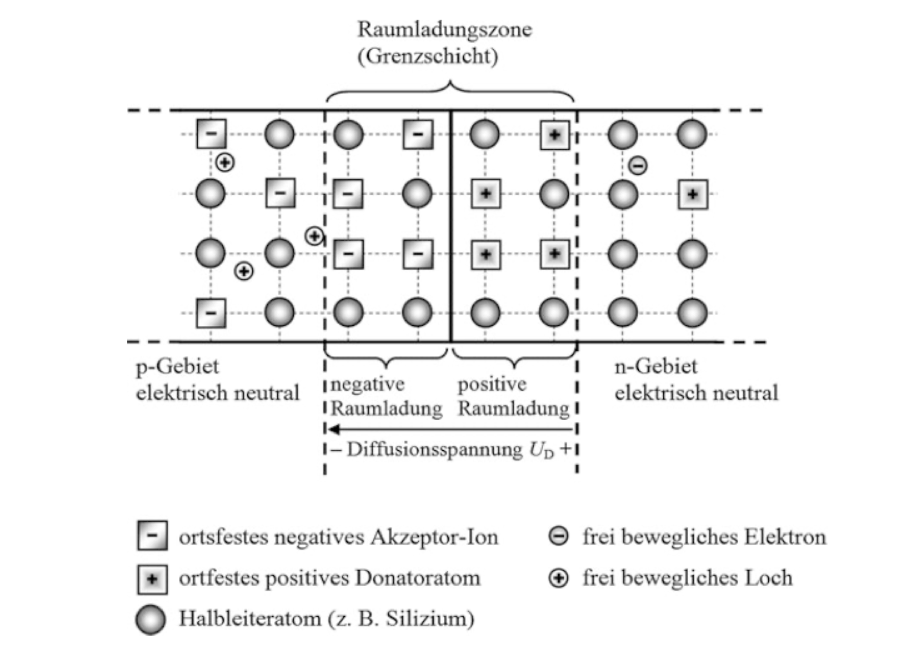
\includegraphics[scale=1]{SperrschichtOhneFreibeweglicheLadungstraeger.png}
\caption{Sperrschicht ohne freibewegliche Ladungsträger \cite{Stiny2018}}
\end{figure}


Das elektrische Feld wirkt dem Diffusionsstrom entgegen, und verhindert ein weiteres Ausbreiten der Raumladungszone. Ohne äußere Einflüsse ist eine Ladungsträgerbewegung über die Grenzschicht nicht mehr möglich. Der zu beiden Seiten hin ungestörte Bereich wird als bulk oder Bahnbereich bezeichnet. Die Diffusionsspannung unterscheidet sich von dem gewählten Halbleitermaterial und ist ein wichtiger Kennwert. Bei Silizium beträgt die Diffusionsspannung ein Wert zwischen $0,6\,V$ und $0,8\,V$.

\section{Diode in Durchlassrichtung} \label{sec:DiodeInDurchlassrichtung}
Ohne angelegte Spannung besitzt die Diode eine Sperrschicht, mit der breite $W_{0}$ , und eine Diffusionsspannung $U_{D}$. Die Sperrschicht beinhaltet keine freibeweglichen Ladungsträger. Es kann kein Ladungsträgerfluss stattfinden. Es wird nun eine externe Gleichspannung $U_{F}$ an der Diode angeschlossen, die in ihrer Richtung der Diffusionsspannung entgegengesetzt ist. Das bedeutet wir schließen  den p-Leiter an den positiven Pol der Spannungsquelle an und den n-Leiter an den negativen Pol. Sobald die äußere Spannung $U_{F}$ größer ist als die Diffusionsspannung $U_{D}$ werden die positiven Ladungsträger aus der p-Schicht in Richtung Minuspol der Spannungsquelle, sprich in Richtung der Sperrschicht gestoßen, und die negativen Ladungsträger aus der n-Schicht in Richtung Pluspol der Spannungsquelle, somit auch ich Richtung der Sperrschicht bewegt. Treffen die positiven und negativen Ladungsträger aufeinander besetzten die freien Elektronen die Löcher, man spricht von einer Rekombination. Die Diffusionsspannung $U_{D}$ wird auf Grund der externen Spannung $U_{F}$ kleiner. Somit verringert sich auch die Breite der Sperrschicht $W_{0}$. In der Abbildung 3 als $U_{DF}$ und $W_{F}$ gekennzeichnet. 

\begin{figure}[!htb]
\centering
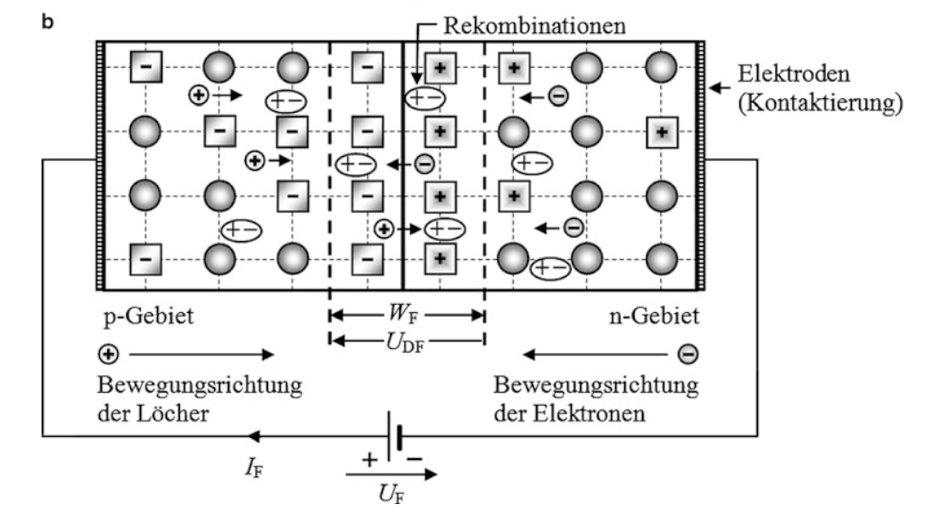
\includegraphics[scale=0.8]{pnUebergangDurchlass.png}
\caption{pn-Übergang in Durchlassrichtung \cite{Stiny2018}}
\end{figure}

Die Sperrschicht $W_{F}$ ist durch die angelegte Spannung so schmal, das Ladungsträger sie durchqueren können. Die Diode wird leitend es fließt ein Durchlassstrom $I_{F}$ . Der Durchlassstrom Steigt zunächst exponentiell mit der angelegten Spannung $U_{F}$, bei zunehmender Spannung stellt sich jedoch eine lineare Abhängigkeit ein. Um die Diode nicht zu beschädigen muss sie mit einem Vorwiderstand $R_{v}$ abgesichert werden. Die Abhängigkeit zwischen $U_{F}$ und $I_{F}$ stellt die Durchlasskennlinie da, mit deren Hilfe man die Schleusenspannung $U_{s}$ bestimmen kann. Die Schleusenspannung gibt Auskunft darüber ab wann die Diode leitend wird. $U_{s}$ kann aus der Durchlasskennlinie abgelesen werden, indem die Tangente des linearen Bereiches auf die Abszisse verlängert wird. 

\begin{figure}[!htb]
\centering
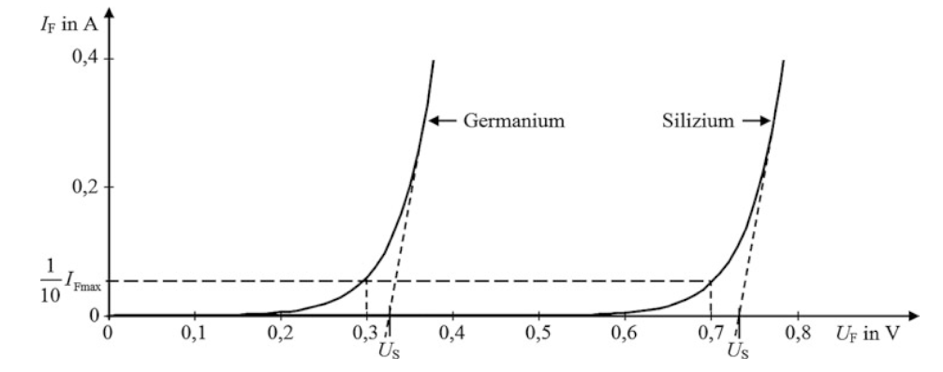
\includegraphics[scale=1]{DurchlasskennlinieGeSiDiode.png}
\caption{Durchlasskennlinie von Ge- und Si-Dioden \cite{Stiny2018}}
\end{figure}

\section{Diode in Sperrrichtung}
Schließt man den negativen Pol der Spannungsquelle an die p-Schicht der Diode, und den positiven Pol an die n-Schicht, so ist die Diode in Sperrrichtung geschaltet. Die Angelegte äußere Spannung stimmt mit ihrer Richtung mit der inneren Diffusionsspannung überein. Die Sperrschicht $W_{0}$ verbreitert sich und verarmt an freien Ladungsträgern, da die Defektelektronen von dem negativen Pol der Spannungsquelle angezogen werden, und die Elektronen von dem positiven Pol. Durch die Verarmung an freien Ladungsträgern steigt der Widerstand. Durch die Diode kann kein Strom fließen, bis auf den vernachlässigbar kleine Sperrstrom der sich im Pikoampere Bereich befindet. Die Diode kann nur einer begrenzten Spannung in Sperrrichtung ausgesetzt werden. Wird ein kritischer Spannungswert überschritten, beschleunigt das elektrische Feld die freien Ladungsträger so sehr, das ihre Energie ausreicht um andere Elektronenpaarbindungen aufzubrechen. Die neuen freibeweglichen Ladungsträger werden auch durch das elektrische Feld beschleunigt und erzeugen wiederum neue freie Elektronen. Man spricht von einem Lawinendurchbruch. Der Sperrstrom steigt schlagartig, wird dieser nicht durch einen entsprechenden vorwiderstand begrenzt, wird die zulässige Leistung der Diode überschritten, sie geht kaputt. 

\begin{figure}[!htb]
\centering
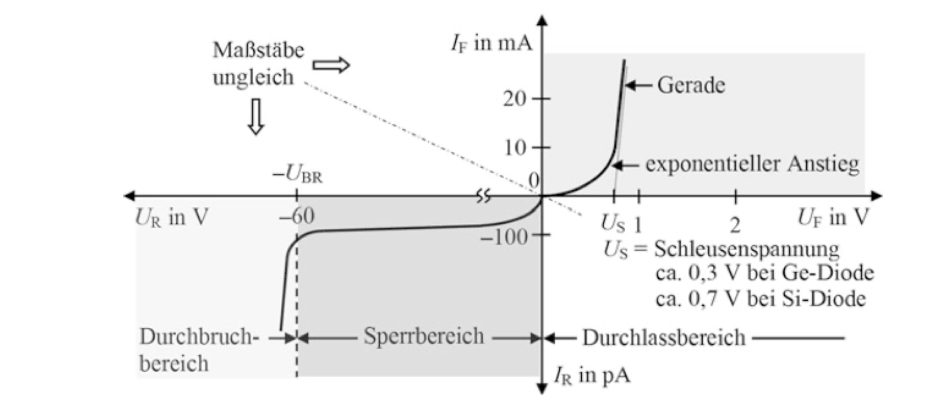
\includegraphics[scale=1]{StromSpannungsKennlinieDiode.png}
\caption{vollständige Strom- Spannungs- Kennlinie einer Diode \cite{Stiny2018}}
\end{figure}

